
\documentclass[conference]{IEEEtran}
\usepackage[left=1.62cm,right=1.62cm,top=1.9cm]{geometry}


% chktex-file 10
% chktex-file 17
% chktex-file 36
% chktex-file 8
% chktex-file 1
% chktex-file 9

\usepackage[english]{babel}
\usepackage{amsmath,amssymb}
\usepackage{times}
\usepackage{relsize}
\usepackage{graphicx}
\usepackage{url}
\usepackage{booktabs}
\usepackage{multirow}
\usepackage{mparhack}
\usepackage{subfigure}
\usepackage{authblk}
\usepackage{amsthm}
\usepackage{mathrsfs}
\usepackage{pgfplots}
\pgfplotsset{width=7cm,compat=1.8}




\usepackage[noend]{algorithmic}
\usepackage[linesnumbered,ruled,vlined]{algorithm2e}
\usepackage{setspace}
\usepackage{cite}

\usepackage{footmisc}
\usepackage{array}
\usepackage{eqparbox}
\usepackage{tikz}

\usepackage{xcolor}
\usepackage{fontawesome}


%========================
\usepackage{mathtools}
\usepackage{bm}
\usepackage[all]{xy}
\usepackage{etoolbox}
\AtBeginEnvironment{figure}{\setcounter{subfigure}{0}}% Resets subfigure counter at start of figure environment
%========================

\usepackage[acronym]{glossaries}
\usepgfplotslibrary{fillbetween}





\DeclarePairedDelimiter\abs{\lvert}{\rvert}%
\DeclarePairedDelimiter\norm{\lVert}{\rVert}%
%========================

\usepackage{accents}
% \newcommand\undercirc[1]{\underaccent{\overcirc}{#1}}

\newcommand\overplus[1]{\accentset{+}{#1}}
\newcommand\overminus[1]{\accentset{-}{#1}}

\newcommand\overcirc[1]{\accentset{\circ}{#1}}
\newcommand\undercirc[1]{\underaccent{\circ}{#1}}

\newtheorem{theorem}{Theorem}
\newtheorem{corollary}{Corollary}
\newtheorem{proposition}{Proposition}

% \theoremstyle{remark}
\newtheorem{lemma}{Lemma}
\newtheorem{remark}{Remark}
\newtheorem{definition}{Definition}
\newtheorem{notation}{Notation}

% \newtheorem{remark}{Remark}
% \theoremstyle{plain}
% \newtheorem{theorem}{Theorem}
% \newtheorem{definition}{Definition}
% \newtheorem{lemma}[theorem]{Lemma}
% \newtheorem{proposition}[theorem]{Proposition}
% \newtheorem{corollary}[theorem]{Corollary}
% \newtheorem{property}{Property}

% \newenvironment{proof}[1][Proof]{\begin{trivlist}
% \item[\hskip \labelsep {\bfseries #1}]}{\end{trivlist}}
% \newenvironment{definition}[1][Definition]{\begin{trivlist}
% \item[\hskip \labelsep {\bfseries #1}]}{\end{trivlist}}
% \newenvironment{example}[1][Example]{\begin{trivlist}
% \item[\hskip \labelsep {\bfseries #1}]}{\end{trivlist}}
% \newenvironment{remark}[1][Remark]{\begin{trivlist}
% \item[hskip \labelsep{\bfseries #1}]}{\end{trivlist}}
% \newenvironment{problem}[1][]{\begin{trivlist}
% \item[{\bfseries #1}]}{\end{trivlist}}

\newenvironment{noindlist}
{%
\begin{list}
{\labelitemi}{\leftmargin=0em \itemindent=2.5em}
\end{list}
}



%\newcommand{\qed}{\nobreak \ifvmode \relax \else
%      \ifdim\lastskip<1.5em \hskip-\lastskip
%      \hskip1.5em plus0em minus0.5em \fi \nobreak
%      \vrule height0.75em width0.5em depth0.25em\fi}

\newcommand{\mymarginpar}[1]{\mbox{} \marginpar{#1}
%\if@twoside \ifodd \thepage %\c@page
\marginparsep{25pt}
%\else \marginparsep 50pt \fi \fi
}
% \newcommand{\comment}[1]{\mymarginpar{Comment} \textbf{#1}}

% \newcommand\T{\rule{0pt}{2.4ex}}
% \newcommand\B{\rule[-1.0ex]{0pt}{0pt}}

%\renewcommand\Authfont{\scshape}
\renewcommand\Affilfont{\footnotesize}
\setlength{\affilsep}{0.5em}




\def\B{\mathcal{B}}
\def\R{\mathcal{R}}
\def\I{\mathcal{I}}
\def\J{\mathcal{J}}
\def\T{\mathcal{T}}
\def\C{\mathcal{C}}
\def\G{\mathcal{G}}
\def\u{\mathpzc{u}}
\def\U{\mathcal{U}}
\def\P{\mathcal{P}}
\def\N{\mathcal{N}}
\def\K{\mathcal{K}}
\def\X{\mathcal{X}}

\def\KK{\mathcal{K}^{+}}
\def\KU{\mathcal{K}^{-}}

\newacronym{csi}{CSI}{channel state information}
\newacronym{wmmse}{WMMSE}{weighted minimum mean square error}
\newacronym{sc}{SC}{synthetic control}
\newacronym{ru}{RU}{resource unit}
\newacronym{wsrm}{WSRM}{weighted sum-rate maximization}
\newacronym{ioe}{IoE}{internet of everything}
\newacronym{gnn}{GNN}{graph neural networks}
\newacronym{siso}{SISO}{single-input-single-output}
\newacronym{idi}{IDI}{interference detection and identification}
\newacronym{cca}{CCA}{clear channel assessment}

\newcommand*{\tran}{^{\mkern-1.5mu\mathsf{T}}} % A\tran
\newcommand*{\conj}[1]{\overline{#1}} % \conj{A}
\newcommand*{\hermconj}{^{\mathsf{H}}} % A\hermconj


\DeclareMathOperator{\argmax}{\arg\max}
\DeclareMathOperator{\argmin}{\arg\min}

\renewcommand{\vec}[1]{\mathbf{#1}}




\newcommand*\diff{\mathop{}\!\mathrm{d}}
\newcommand*\Diff[1]{\mathop{}\!\mathrm{d^#1}}
\DeclareMathOperator{\EE}{\mathbb{E}}


% \makeatletter
% \patchcmd{\@maketitle}
%   {\addvspace{0.5\baselineskip}\egroup}
%   {\addvspace{-1.45\baselineskip}\egroup}
%   {}
%   {}
% \makeatother

\title{Weighted Sum-Rate Maximization With Causal Inference for Latent Interference Estimation}


\author[ ]{Lei You}
\affil[ ]{\small Department of Engineering Technology, Technical University of Denmark, Denmark}
\affil[ ]{\text{lei.you@pm.me}}


\begin{document}

\maketitle
\thispagestyle{plain}
\pagestyle{plain}

\begin{abstract}
The paper investigates the \gls{wsrm} problem with latent interfering sources outside the known network, whose power allocation policy is hidden from and uncontrollable to optimization. The paper extends the famous alternate optimization algorithm \gls{wmmse} \cite{christensen2008weighted} under a causal inference framework to tackle with \gls{wsrm} under latent interference. Namely, 
% the optimzer's decision serves as a confounder of the power on latent links and the observed interference of the known network. 
with the possibility of power policy shifting in the hidden network, 
computing an iterating direction based on the observed interference inherently implies that counterfactual is ignored in decision making. A \gls{sc} method is used to estimate the counterfactual. For any link in the known network, \gls{sc} constructs a convex combination of the interference on other links and uses it as an estimate. Power iteration is performed on the estimated rather than the observed interference. The proposed SC-WMMSE requires no more information than its origin. To our best knowledge, this is the first paper explores the potential of \gls{sc} to assist mathematical optimization in addressing classic wireless optimization problems. Numerical results suggest the superiority of the SC-WMMSE over the original in both convergence and objective.
\end{abstract}
\glsresetall

\section{Introduction}
\label{sec:intro}


The wireless network evolution has been driven by a need for higher rates consistently for the past decades together with an emergence of the \gls{ioe}, which aims to serve as a platform to make connections among process, people and data~\cite{saad2019vision}. The requirement on high spectral efficiency in the scenarios of \gls{ioe} calls for a need of revisiting classic wireless optimization problems under highly dynamic environments. The \gls{wsrm} problem \cite{baligh2014cross} is one of these many, solving which plays a key role in determining the effective capacity of a wireless channel. 
Finding the global maximum of \gls{wsrm} is generally $\mathcal{NP}$-hard \cite{baligh2014cross}.

Consequently, research effort has been devoted for high-quality sub-optimal solutions. The \gls{wmmse} algorithm, proposed firstly in~\cite{christensen2008weighted} is one of them which is shown to be an efficient algorithmic framework for many cross-layer transmission tasks \cite{baligh2014cross}. Hence, this algorithmic framework has been extended significantly by many other literature and the research exploring remains still active \cite{schmidt2009minimum, shi2011iteratively, shin2012weighted, cirik2015weighted, aquilina2017weighted, guo2020weighted}. Besides, the \gls{wsrm} problem was also visited by data-driven methodologies--more specifically--\gls{gnn} based methods \cite{eisen2020optimal,naderializadeh2020wireless,chowdhury2021unfolding, nikoloska2021fast}. The basic idea is to use a \gls{gnn} to encode the network topology information into a \gls{gnn} that maps \gls{csi} to power control policy. Unsupervised model training is also possible by in-cooperating learning in the processing of a primal-dual algorithm \cite{eisen2020optimal}. 

The \gls{siso} case of~\cite{schmidt2009minimum, shi2011iteratively, shin2012weighted, cirik2015weighted, aquilina2017weighted, guo2020weighted,eisen2020optimal,naderializadeh2020wireless,chowdhury2021unfolding, nikoloska2021fast} and many other research summarized in \cite{weeraddana2012weighted} falls into a special case of the problem investigated in this paper, i.e. when there is no latent interfering links whose power allocation is unknown and uncontrollable. Under this setup, the paper inspects the \gls{wmmse} optimization mechanism via a causal inference's perspective. The \gls{wmmse} algorithm or similar other iterative methods suffer performance loss on the new setup due to the overlook of the influence from latent factor on the iterating directions (gradient, sub-gradient etc.) towards the ground-truth optimality. For the links in the known network, \textit{the causality between power and the interference is difficult to formulate in an accurate and exact way}. The paper proposes a variant of it leveraging\gls{sc} method \cite{abadie2003economic} for causality identification. Namely, the \gls{sc} method estimates the counterfactual which is then used by the optimizer to infer the causality relationship between optimization variables and the objective (and, equivalently, the ground truth formulation). The proposed algorithm is named SC-WMMSE. Remark that SC-WMMSE requires no more information of the network than the original \gls{wmmse} and hence the trick in this paper applies to most of its previous extensions \cite{baligh2014cross,schmidt2009minimum, shi2011iteratively, shin2012weighted, cirik2015weighted, aquilina2017weighted, guo2020weighted}. Numerically, the proposed SC-WMMSE shows advantage over its origin on both convergence and objective value as well as demonstrates resilience to emerging and disappearing of latent interference sources.



\begin{figure*}[!t]
\begin{equation}
R_k = \log\bigg(1+\frac{|h_{k,k}|^2 p_k}{\sum_{j\in\KK}|h_{j,k}|^2p_j +\sum_{i\in\KU}|h_{i,k}|^2q_i+ \sigma^2_k }\bigg)\quad k\in\KK
\label{eq:KK_rate}
\end{equation}
\end{figure*}

\section{Model and Problem}



Consider a wireless network consisting of multiple communications links. Denote by $\K$ the set of all links. For any link $k$ ($k\in\K$), denote by $\I_k$ the set of links interfering with $k$, $\I_k\subseteq \K$. Denote by $h_{k,k}$ the channel gain between the transmitter and the receiver of link $k$ ($k\in\K$). Similarly, denote by $h_{k,j}$ ($k\neq j$) the channel gain from the transmitter of link $k$ and the receiver of link $j$. For simplicity, let $|h_{k,j}|=0$ for any $j\notin \I_k$ ($j\neq k$). Denote by $\vec{H}$ the channel matrix. Denote by $p_k$ the power of the transmitter of link $k$ ($k\in\K$). 
Denote $\sigma_k^2$ the noise power. 
The aim is to find a power allocation $p_1,p_2\ldots p_K$ of all the corresponding transmitters of the $K$ links such that the weighted sum rate $\sum_{k}\alpha_k R_k$ is maximized.


% \subsection{Preliminaries}

% The \textit{classic} weighted sum-rate maximization problem is formulated in~\eqref{eq:opt_naive} below.
% \begin{subequations}
% \begin{align}
%                  & \max_{\vec{p}} \sum_{k=1}^{K}\alpha_k \mathbb{E}_{\vec{H}}\bigg[\log\left(1+\frac{|h_{k,k}|^2 p_k}{\sum_{j\in\K}|h_{j,k}|^2p_j + \sigma^2_k }\right)\bigg] \\
% \text{s.t.}\quad & 0\leq p_{k}\leq p_k^{\max},~k=1,2,\ldots K
% \end{align}
% \label{eq:opt_naive}
% \end{subequations} 

Consider there are latent interference sources whose power distribution is not known a prior and power allocation is neither observable nor controllable. Denoted by $\KK$ and $\KU$ respectively the known and the unknown networks and let $K=|\KK|$. Remark $\KK\cap\KU=\phi$ and $\KK\cup\KU=\K$. Note that $\KK$ and $\KU$ mutually affect each other via interference.

There is no assumption imposed on $\KU$ regarding its power policies. Namely, the policies could proactively or reactively change/switch across time. The notation $\vec{q}$ is used to represent the power allocation in $\KU$ so as to distinguish with the power allocation $\vec{p}$ in $\KK$. The problem is defined in~\eqref{eq:opt} below, with $R_k$ defined in \eqref{eq:KK_rate}.

% The problem in \eqref{eq:opt_naive} is generalized to~\eqref{eq:opt} below. Remark that the formulation~\eqref{eq:opt_naive} is a special case of~\eqref{eq:opt}. Setting $\KU=\phi$ reduces the inner statistical expectation such that the objective function degenerates to the one in~\eqref{eq:opt_naive}. 
\begin{subequations}
\begin{align}
                 & \max_{\vec{p}} \sum_{k\in\KK}\alpha_k\mathbb{E}_{\vec{H}}\bigg[\mathbb{E}_{\vec{q}|\vec{H}}\big[ R_k\big] \bigg]\\
\text{s.t.}\quad & 0\leq p_{k}\leq p_k^{\max},~k\in\KK
\end{align}
\label{eq:opt}
\end{subequations} 


% Inspecting the formulation, the inner mathematical expectation $\mathbb{E}_{\vec{q}|\vec{H},\vec{p}}$ imposes that the power allocation $\vec{q}$ is conditional on the power allocation $\vec{p}$. First, it means $\KK$ needs to be optimized by taking into account the power allocation of $\KU$, though the allocation policy of $\KU$ is not known. Additionally, one cannot expect to sampling on the environment to learn a conditional distribution $\P(\vec{q}|\vec{H})$ to ease the optimization. This is because $\vec{q}$ is conditionally distributed on both $\vec{p}$ and $\vec{H}$, such that any change of $\vec{p}$ from the optimization would lead to a  distribution drifting on $\P(\vec{q}|\vec{H})$. 

% Note that the widely investigated distributed optimization techniques for solving~\eqref{eq:opt_naive} do not generalize to solving~\eqref{eq:opt}. In those research, though the power can be optimized in a distributed manner and gets updated asynchronously in each sub-network, it is required that each sub-network is aware of the existing of others and all sub-networks are subject to the same power optimization policy. Essentially, it means that the power allocations of all sub-networks needs to follow the same optimization policy. Sub-networks targeting at a different objective or employing various power allocation polices cannot be put into those optimization frameworks.







\section{Sum Rate Maximization with Causal Inference}
\label{sec:sum-rate}

% This section illustrates how \gls{wmmse} may go biased from the optimization target in its inherent optimization mechanism. Then, the how a causal estimator differs with a regression estimator is discussed in the scope of extending \gls{wmmse} with interference estimation for solving~\eqref{eq:opt}. Next, \gls{sc} is introduced to establish a causal estimator that can be trained offline in low cost and Incorporated to \gls{wmmse}, followed by the algorithm design of SC-WMMSE.


\subsection{How Latent Interference Affects \gls{wmmse}}
\label{subsec:wmmse}

It is shown that~\eqref{eq:opt} submits to a reformulation as a weighted sum-mean-square-error minimization problem \cite{schmidt2009minimum,shi2011iteratively} when $\vec{q}$ is fixed as constants. Let $\vec{q}$ be fixed in~\eqref{eq:opt} such that the mathematical expectation on $\vec{q}$ diminishes. 
Denote 
$\eta_{k}=\sum_{i\in\KU}|h_{i,k}|^2q_i + \sigma^2_k$.
Replacing the noise plus the interference term from $\KU$ by $\eta_k$ in the denominator of \eqref{eq:KK_rate}, the formulation~\eqref{eq:opt} can hence can be re-written as~\eqref{eq:opt_naive_reform} without loss of optimality. 

\begin{subequations}
\begin{align}
                 & \min_{\vec{w}, \vec{u}, \vec{v}} \mathbb{E}_{\vec{H}}\bigg[ \sum_{k\in\KK} \alpha_k(w_{k}e_k - \log w_k)\bigg] \\
\text{s.t.}  \quad& \lvert v_{k}\rvert^2 \leq p^{\max}_k,~k\in\KK
\end{align}
\label{eq:opt_naive_reform}
\end{subequations} 

The variable $w_k$ is a positive weight variable and the variable $e_k$ is the mean-square estimation error, defined as follows. This reformulation is shown to share the same optimum of~\eqref{eq:opt}.
\begin{equation}
e_k = |u_k h_{k,k}, v_k - 1|^2 + \sum_{j\neq k}|u_j h_{j,k}v_k|^2 +g_{k}|u_k|^2
\end{equation}
The \gls{wmmse} algorithm is designed under the classical theory of alternate optimization to solve the formulation~\eqref{eq:opt_naive_reform}, illustrated in Algorithm~\ref{alg:wmmse}\footnote{Remark that \gls{wmmse} has its stochastic version, which is designed to deal with the case that $\vec{H}$ is a random variable, e.g. \eqref{eq:opt_naive_reform}. The difference to the deterministic version is that the numerator and denominator of $v_k$ is accumulated respectively over iterations. The variable $v_k$ gets updated by the accumulated values rather than the single-sample values in each iteration. The proposed methodology in this paper generalizes straightforwardly to the stochastic version of \gls{wmmse}\label{footnote:stochastic_wmmse}}. Practically, $\eta_{k}$ needs to be obtained in approximation by \gls{idi} techniques such as \gls{cca} \cite{yang2011wireless}.

\begin{algorithm}
\setstretch{1.25}
\caption{The \gls{wmmse} algorithm for solving the problem in~\eqref{eq:opt_naive_reform}.}
\label{alg:wmmse}
\begin{algorithmic}[1]
\STATE Initialize $\vec{v}, \vec{u}, \vec{w}$ randomly
\REPEAT 
    \STATE Observe $\eta_1, \eta_2\ldots \eta_{K}$ \label{alg:1-gk}
  \FORALL{$k = 1, 2\ldots K$}
    \STATE $u_k = |h_{k,k}v_k| / (\sum_{j\in\KK}|h_{j,k}|^2|v_j|^2 + \eta_k )$ \label{alg:1-u_k}
    \STATE $w_k = 1 / (1 - |u_k h_k v_k|)$
    \STATE $v_k = \alpha_k h_k u_k w_k / (\sum_{j\in\KK}\alpha_jw_j |h_{k,j}u_j|^2 + \lambda_k)$
  \ENDFOR
\UNTIL \text{Convergence}
\RETURN $\vec{v},\vec{u},\vec{w}$
\end{algorithmic}
\end{algorithm}

The term $e_k$ is a convex quadratic function over $\vec{u}$ and $\vec{v}$. These variables are subject to a closed form solution, with $\lambda_k$ subject to bisection search to make $v_k$ satisfy its power constraint. Now consider the case that $\vec{q}$ is a latent random variable rather than staying fixed, whose distribution is unobserved. This change influences the behavior of Algorithm~\ref{alg:wmmse} in Line~\ref{alg:1-u_k}.
% Namely, $\eta_{k}$ is a random variable rather than a constant. 
% Note that \gls{wmmse} has its stochastic version to deal with randomization on $\vec{H}$ (see footnote\footref{footnote:stochastic_wmmse}). 
Once the power policy that yields $\vec{q}$ change or switch throughout the optimization, the sampling on $\eta_k$ is non-i.i.d throughout the process of Algorithm~\ref{alg:wmmse}, creating challenges for stochastic optimization. Namely, once the algorithm would like to perform iterations based on observations, i.e. updating $u_k$, the collected samples $\eta_k$ ($k\in\K$) does not necessarily guarantee that $u_k$ goes towards the optimum of the quadratic function $e_k$ (given fixed $\vec{w}$). This problem diminishes if $\eta_k$ is i.i.d.

\subsection{Causal Inference Estimator vs. Regression Estimator}
\label{subsec:causal_vs_reg}
\label{subsec:opt-formulation}
As discussed, the key obstacle of applying \gls{wmmse} lies on the fact that the interference at any receiver $k$ ($k\in\KK$) is difficult to handle from optimization's perspective, due to the dependency of $\eta_{k}$ on $\vec{q}$ of which the distribution may shift across time. This subsection gives a discussion on potential methodologies for tackling this obstacle. 

Rather than consider only $\eta_{k}$, we consider the entire denominator of $u_k$, denote by $I_{k}$. The purpose is to make the later proposed inference methodology to generalize better. Namely, for any link $k$, if the \gls{csi} of another link $j$ ($j\neq k$, $j\in\KK$) is unknown or outdated, the proposed inference methodology could estimate the denominator as a whole. The mathematical expectation of $I_k$ is computed as follows.
\begin{equation*}
\begin{split}
   \MoveEqLeft  \mathbb{E}[I_{k}(\vec{p})] \\ 
    \!\!={}& \mathbb{E}_{\vec{H}}\mathbb{E}_{\vec{q}|\vec{H}}\bigg[\sum_{j\in\KK}\!\!|h_{j,k}|^2p_j + \sum_{i\in\KU}\!\!|h_{i,k}|^2q_ik + \sigma_k^2\bigg]  \\
    \!\!={}& \mathbb{E}_{\vec{H}}\bigg[\!\sum_{j\in\KK}\!\!|h_{j,k}|^2p_j\bigg] + \underbrace{\mathbb{E}_{\vec{H}}\mathbb{E}_{\vec{q}|\vec{H}}\bigg[\!\sum_{i\in\KU}\!\!\!|h_{i,k}|^2q_i+\sigma_k^2\bigg]}_{\eta_{k}}
\end{split}
\end{equation*}

Note that $\mathbb{E}[I_k(\vec{p})]$ decomposes to two parts. The first part can be accurately computed if \gls{csi} of $\KK$ is known. Estimating the second part $\eta_{k}$ is tricky. Supervised machine learning models are not practical for this task due to that any power policy change of $\KU$ leads to the violation of i.i.d assumption for training. Once the power allocation policy changed in $\KU$ or transmitters/receivers join/leave the sub-network of $\KU$, the distribution $\P(\vec{q}|\vec{H})$ may drift from the originally learned one. 

Causal inference estimates the potential outcome of the interference in reaction to its power allocation decision taking into consideration the counterfactual. Namely, for every power allocation $\vec{p}$ applied to the network, we could only observe the network's responded $I_k$, but never gets a chance to observe the effect of assigning a power other than $\vec{p}$. With a shift on $\KU$'s power policy, an estimator that gives estimation for  $\mathbb{E}[I_k|\vec{p}]$ would be biased. This is usually what an regression estimator does, i.e. computing the statistical mean on observational data. A causal inference estimator is different in targeting $\mathbb{E}[I_k|do(\vec{p})]$ rather than the statistical mean, where the \textit{do}-operator represent an intervention of power allocation $\vec{p}$ on the whole population of covariates (all candidate power policies of $\KU$ in this context) rather than any observed proportion of the whole. In other words, $\mathbb{E}[I_k|do(\vec{p})]$ takes both the fact and the counterfactual into consideration. The optimization direction of $\vec{p}$ (e.g. gradient, sub-gradient, or other directions) needs to be constructed based $\mathbb{E}[I_k|do(\vec{p})]$ rather than $\mathbb{E}[I_k|\vec{p}]$ given the possibility of the change of $\vec{q}$'s distribution. An estimator that does $\mathbb{E}[I_k|do(\vec{p})]$ rather than $\mathbb{E}[I_k|\vec{p}]$  leads to the yielded solutions generalize better. In the next section it is shown that the desired estimation can be obtained from observational data also, rather than doing intervention on the whole population.


% , so as to justify the iteration direction of the variable $\vec{p}$. The variable $\vec{q}$ that influences both $p_k$ and $I_k$ ($k\in\KK$), the estimation is towards the outcome of $\mathbb{E}[I_k|do(\vec{p})]$ rather than the statistical mean $\mathbb{E}[I_k|\vec{p}]$ computed on any observational datasets. In other words, the optimization direction of $\vec{p}$ (e.g. gradient, sub-gradient, or other directions) needs to be constructed based on both the factual and the counterfactual outcomes, whereas the latter is always missing in observational data. The major difference is that $\mathbb{E}[I_k|\vec{p}]$ is calculated on the observed data which is only parts of the whole population of its covariates while $\mathbb{E}[I_k|do(\vec{p})]$ is on the whole.  Nevertheless, in the next section it is shown that the desired estimation can be obtained from observational data by a causal inference estimator.


\subsection{Estimating Interference with \gls{sc} Methods}
\label{subsec:sc}


\begin{figure}
\centering
\tikzset{every picture/.style={line width=0.75pt}} %set default line width to 0.75pt          

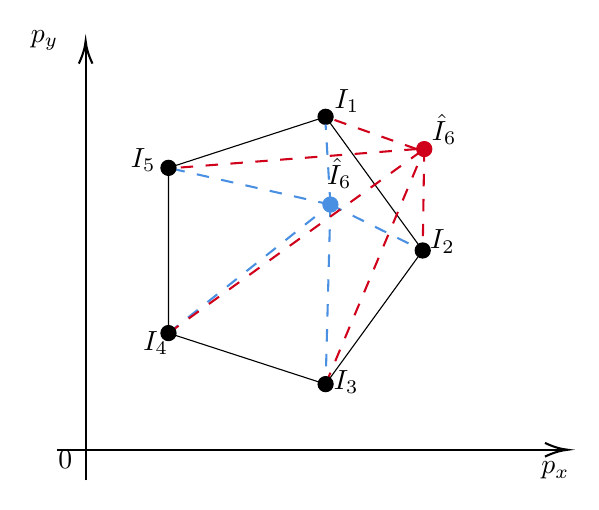
\begin{tikzpicture}[x=0.75pt,y=0.75pt,yscale=-1,xscale=1]
%uncomment if require: \path (0,847); %set diagram left start at 0, and has height of 847

%Shape: Polygon [id:dp224164202141931] 
\draw   (366.92,228.47) -- (320.13,292.88) -- (244.42,268.28) -- (244.42,188.67) -- (320.13,164.07) -- cycle ;
%Shape: Ellipse [id:dp3256341156223599] 
\draw  [color={rgb, 255:red, 208; green, 2; blue, 27 }  ,draw opacity=1 ][fill={rgb, 255:red, 208; green, 2; blue, 27 }  ,fill opacity=1 ] (364.01,179.62) .. controls (364.01,177.61) and (365.65,175.98) .. (367.66,175.98) .. controls (369.67,175.98) and (371.3,177.61) .. (371.3,179.62) .. controls (371.3,181.63) and (369.67,183.26) .. (367.66,183.26) .. controls (365.65,183.26) and (364.01,181.63) .. (364.01,179.62) -- cycle ;
%Straight Lines [id:da8764490533518536] 
\draw [color={rgb, 255:red, 74; green, 144; blue, 226 }  ,draw opacity=1 ][line width=0.75]  [dash pattern={on 4.5pt off 4.5pt}]  (322.45,206.36) -- (366.92,228.47) ;
%Straight Lines [id:da6851668490079947] 
\draw [color={rgb, 255:red, 74; green, 144; blue, 226 }  ,draw opacity=1 ][line width=0.75]  [dash pattern={on 4.5pt off 4.5pt}]  (322.45,206.36) -- (320.13,292.88) ;
%Straight Lines [id:da23609417084914575] 
\draw [color={rgb, 255:red, 74; green, 144; blue, 226 }  ,draw opacity=1 ][line width=0.75]  [dash pattern={on 4.5pt off 4.5pt}]  (244.42,268.28) -- (322.45,206.36) ;
%Straight Lines [id:da2571972397860731] 
\draw [color={rgb, 255:red, 74; green, 144; blue, 226 }  ,draw opacity=1 ][line width=0.75]  [dash pattern={on 4.5pt off 4.5pt}]  (322.45,206.36) -- (244.42,188.67) ;
%Straight Lines [id:da2251639682861042] 
\draw [color={rgb, 255:red, 208; green, 2; blue, 27 }  ,draw opacity=1 ][line width=0.75]  [dash pattern={on 4.5pt off 4.5pt}]  (320.13,292.88) -- (367.66,179.62) ;
%Straight Lines [id:da7789718802550452] 
\draw [color={rgb, 255:red, 208; green, 2; blue, 27 }  ,draw opacity=1 ][line width=0.75]  [dash pattern={on 4.5pt off 4.5pt}]  (244.42,268.28) -- (367.66,179.62) ;
%Straight Lines [id:da23249730714159367] 
\draw [color={rgb, 255:red, 208; green, 2; blue, 27 }  ,draw opacity=1 ][line width=0.75]  [dash pattern={on 4.5pt off 4.5pt}]  (367.66,179.62) -- (366.92,228.47) ;
%Straight Lines [id:da6827372695149887] 
\draw [color={rgb, 255:red, 208; green, 2; blue, 27 }  ,draw opacity=1 ][line width=0.75]  [dash pattern={on 4.5pt off 4.5pt}]  (364.01,179.62) -- (320.13,164.07) ;
%Shape: Ellipse [id:dp7050237810455391] 
\draw  [fill={rgb, 255:red, 0; green, 0; blue, 0 }  ,fill opacity=1 ] (363.28,228.47) .. controls (363.28,226.46) and (364.91,224.83) .. (366.92,224.83) .. controls (368.93,224.83) and (370.56,226.46) .. (370.56,228.47) .. controls (370.56,230.49) and (368.93,232.12) .. (366.92,232.12) .. controls (364.91,232.12) and (363.28,230.49) .. (363.28,228.47) -- cycle ;
%Shape: Ellipse [id:dp9309501596310132] 
\draw  [fill={rgb, 255:red, 0; green, 0; blue, 0 }  ,fill opacity=1 ] (316.49,164.07) .. controls (316.49,162.06) and (318.12,160.43) .. (320.13,160.43) .. controls (322.14,160.43) and (323.77,162.06) .. (323.77,164.07) .. controls (323.77,166.09) and (322.14,167.72) .. (320.13,167.72) .. controls (318.12,167.72) and (316.49,166.09) .. (316.49,164.07) -- cycle ;
%Shape: Ellipse [id:dp7614343877717125] 
\draw  [fill={rgb, 255:red, 0; green, 0; blue, 0 }  ,fill opacity=1 ] (240.78,188.67) .. controls (240.78,186.66) and (242.41,185.03) .. (244.42,185.03) .. controls (246.43,185.03) and (248.07,186.66) .. (248.07,188.67) .. controls (248.07,190.68) and (246.43,192.32) .. (244.42,192.32) .. controls (242.41,192.32) and (240.78,190.68) .. (240.78,188.67) -- cycle ;
%Shape: Ellipse [id:dp936113035140345] 
\draw  [fill={rgb, 255:red, 0; green, 0; blue, 0 }  ,fill opacity=1 ] (240.78,268.28) .. controls (240.78,266.26) and (242.41,264.63) .. (244.42,264.63) .. controls (246.43,264.63) and (248.07,266.26) .. (248.07,268.28) .. controls (248.07,270.29) and (246.43,271.92) .. (244.42,271.92) .. controls (242.41,271.92) and (240.78,270.29) .. (240.78,268.28) -- cycle ;
%Shape: Ellipse [id:dp14199884674981345] 
\draw  [fill={rgb, 255:red, 0; green, 0; blue, 0 }  ,fill opacity=1 ] (316.49,292.88) .. controls (316.49,290.86) and (318.12,289.23) .. (320.13,289.23) .. controls (322.14,289.23) and (323.77,290.86) .. (323.77,292.88) .. controls (323.77,294.89) and (322.14,296.52) .. (320.13,296.52) .. controls (318.12,296.52) and (316.49,294.89) .. (316.49,292.88) -- cycle ;
%Shape: Ellipse [id:dp35213262674036416] 
\draw  [color={rgb, 255:red, 74; green, 144; blue, 226 }  ,draw opacity=1 ][fill={rgb, 255:red, 74; green, 144; blue, 226 }  ,fill opacity=1 ] (318.8,206.36) .. controls (318.8,204.35) and (320.43,202.72) .. (322.45,202.72) .. controls (324.46,202.72) and (326.09,204.35) .. (326.09,206.36) .. controls (326.09,208.38) and (324.46,210.01) .. (322.45,210.01) .. controls (320.43,210.01) and (318.8,208.38) .. (318.8,206.36) -- cycle ;
%Straight Lines [id:da36974497752955027] 
\draw [line width=0.75]    (190.8,324.49) -- (434.77,324.49) ;
\draw [shift={(436.77,324.49)}, rotate = 180] [color={rgb, 255:red, 0; green, 0; blue, 0 }  ][line width=0.75]    (10.93,-3.29) .. controls (6.95,-1.4) and (3.31,-0.3) .. (0,0) .. controls (3.31,0.3) and (6.95,1.4) .. (10.93,3.29)   ;
%Straight Lines [id:da37889403281928824] 
\draw [line width=0.75]    (204.52,339.19) -- (204.52,129.52) ;
\draw [shift={(204.52,127.52)}, rotate = 90] [color={rgb, 255:red, 0; green, 0; blue, 0 }  ][line width=0.75]    (10.93,-3.29) .. controls (6.95,-1.4) and (3.31,-0.3) .. (0,0) .. controls (3.31,0.3) and (6.95,1.4) .. (10.93,3.29)   ;
%Straight Lines [id:da8075828784484049] 
\draw [color={rgb, 255:red, 208; green, 2; blue, 27 }  ,draw opacity=1 ][line width=0.75]  [dash pattern={on 4.5pt off 4.5pt}]  (364.01,179.62) -- (248.07,188.67) ;
%Straight Lines [id:da06190541080915435] 
\draw [color={rgb, 255:red, 74; green, 144; blue, 226 }  ,draw opacity=1 ][line width=0.75]  [dash pattern={on 4.5pt off 4.5pt}]  (322.45,206.36) -- (320.13,167.72) ;

% Text Node
\draw (323.23,149.49) node [anchor=north west][inner sep=0.75pt]  [font=\normalsize]  {$I_{1}$};
% Text Node
\draw (369.25,217.36) node [anchor=north west][inner sep=0.75pt]  [font=\normalsize]  {$I_{2}$};
% Text Node
\draw (322.86,285.22) node [anchor=north west][inner sep=0.75pt]  [font=\normalsize]  {$I_{3}$};
% Text Node
\draw (231.06,266.42) node [anchor=north west][inner sep=0.75pt]  [font=\normalsize]  {$I_{4}$};
% Text Node
\draw (225.1,177.92) node [anchor=north west][inner sep=0.75pt]  [font=\normalsize]  {$I_{5}$};
% Text Node
\draw (319.55,182.82) node [anchor=north west][inner sep=0.75pt]  [font=\normalsize]  {$\hat{I}_{6}$};
% Text Node
\draw (370.06,161.75) node [anchor=north west][inner sep=0.75pt]  [font=\normalsize]  {$\hat{I}_{6}$};
% Text Node
\draw (422.83,329.15) node [anchor=north west][inner sep=0.75pt]    {$p_{x}$};
% Text Node
\draw (176.86,121.4) node [anchor=north west][inner sep=0.75pt]    {$p_{y}$};
% Text Node
\draw (190.14,323.58) node [anchor=north west][inner sep=0.75pt]    {$0$};


\end{tikzpicture}
\caption{Illustration of interpolation vs. extrapolation. Consider $\KK=\{1,2,3,4,5,6\}$ and $\KU=\{x,y\}$. Note that $q_x$ and $q_y$ are latent variables to $\KK$, influencing the observed interference at each link of $\KK$. The positions of $I_1,I_2\ldots I_5$ are affected by the value of $q_x$ and $q_y$ at the moment of observation. Estimations are performed for the link $6$, denoted by $\hat{I}_6$ with blue and red dots. The blue is from intertropolation, as it falls in-between the known observations (i.e. the convex hull), whereas the red is from extrapolation. }
\label{fig: constrained_lr}
\end{figure}



% Recall that the problem faced in \gls{wmmse} is that the power allocation $\vec{q}$ of the sub-network $\KU$ stays latent and serve as a confounding variable influencing both the treatment $\vec{p}$ (because the algorithm generating the treatment depends on $\vec{q}$ via the term $\eta_{k}$) and the observation $I_k$ (by $I_k$'s expression). Consequently, the sampled data may not be able to uncover the truth of the environment so that the power allocation is not optimized towards the desired maximization goal, namely, $\mathbb{E}_{\vec{q}|\vec{p}}[R_k]$ over the entire population of $\vec{p}$ rather than one with $\vec{p}$ constrained in some limited space.

\gls{sc} methods, originally proposed in \cite{abadie2003economic}, have been widely used to estimate the effect caused by a large-scale intervention \cite{shi2022assumptions} and is shown to be competitive against any fixed matching estimator \cite{chen2022synthetic}. The idea behind \gls{sc} is quite simple: It approximates one unit's counterfactual outcomes by constructing a weighted combination of some other units' observed outcomes. More specifically, \gls{sc} methods work with \textit{panel data}, i.e. the data that contains multiple observations for each unit and each unit is observed across time. Though \gls{sc} is widely applied to the case of binary treatment and no interference between units, its usage is not limited by these setups, see \cite{agarwal2022network} for a similar causal factor model setup with this paper, where the potential outcome for unit $k\in\KK$ is linear to the latent factors, with noise in the factor model being additive, zero mean, and independent.

Following the discussions in Sections~\ref{subsec:wmmse} and~\ref{subsec:causal_vs_reg}, it is shown below how \gls{sc} is used to construct an estimator for $\mathbb{E}[I_k|do(\vec{p})]$ for unit $k$ ($k\in\KK$) on a treatment $\vec{p}$. The training and inference stages are described separately below.

The training process is described as follows. Consider observations of $I_1,I_2\ldots I_k$ in format of panel data, i.e.
\begin{equation*}
\vec{X}=
\begin{bmatrix}
I_1^{(0)} & I_2^{(0)} & \cdots  & I^{(0)}_{K}  \\
I_1^{(1)} & I_2^{(1)} & \cdots  & I^{(1)}_{K}  \\
 \vdots & \vdots  & \ddots & \vdots      \\
I_1^{(L)} & I_2^{(L)} & \cdots  & I^{(L)}_{K}  
\end{bmatrix} \in \mathbb{R}^{L\times K}
\end{equation*}
where each row $\ell$ ($1\leq\ell\leq L$) is an observation across all the $K$ units. For any $k\in\KK$, denote by $\vec{x}_k$ the $k_{\text{th}}$ column of $X$. Denote by $\vec{X}_{-k}$ the matrix without column $k$. The \gls{sc} estimator is trained by solving the constrained optimization problem~\eqref{eq:sc} as follows.
\begin{subequations}
\begin{align}
                 & \bm{\nu}_k = \arg\min_{\bm{\beta}\geq\vec{0}} \| \vec{x}_{k} - \vec{X}_{-k}\bm{\beta}\| \label{eq:sc-obj} \\
\text{s.t.}  \quad& \sum_{i} \beta_i = 1   \quad i=1,2\ldots K-1 \label{eq:sc-constr}
\end{align}
\label{eq:sc}
\end{subequations} 



Solving \eqref{eq:sc} yields a vector $\bm{\nu}_{k}$ ($k\in\KK$), which is essentially a group of coefficients that can be used to construct a linear combination of $I_j$ ($j\in\KK\backslash \{k\}$). The objective function~\eqref{eq:sc-obj} suggests that the computed coefficients lead to an as small as possible mean-squared-error over all the $L$ observations of the unit $k$ and respectively its constructed linear combinations. Note that \eqref{eq:sc-constr} imposes a hard constraint on the coefficients such that the obtained linear combination is guaranteed to be a convex combination. One could relax~\eqref{eq:sc-constr} to the objective function as a soft constraint as a Lasso or Ridge regularization term. In other words, solving the formulation~\eqref{eq:sc} trains a (constrained) linear regression model between the observed interference of unit $k$ and those of the others. In this context, a convex combination has better explainability. Namely, in terms of interference, every the units other than $k$ either positively correlates to $k$, or independent to $k$. This is also referred to as interpolation as opposed to extrapolation. See \figurename~\ref{fig: constrained_lr} for an illustration. Section~\ref{sec:simulation} demonstrates the necessity of constraint~\eqref{eq:sc-constr} by showing numerically it helps improving optimization significantly.

Consider the inference stage. Let $\bm{\mu}_{k}$ denotes the observations for all units other than $k$. It is worth noting that $\mu_{k}$ may be drawn from a different distribution than $\vec{X}$, due to the power policy change of $\KU$. The effectiveness of the proposed method in such i.i.d cases is demonstrated in Section~\ref{sec:simulation}. The inference is done simply by $\hat{I}_k = \bm{\nu}_k^{\intercal}\bm{\mu}_k$ for all $k\in\KK$.

\subsection{Algorithm Design}
\label{subsec:sc-wmmse}


\begin{figure*}[t]
\centering

\subfigure[$|\KU|=20$\label{fig:dep-dep-k20}]{
\begin{tikzpicture}
\begin{axis}[
    ymin=120, 
    xlabel={Iterations},
    ylabel={Giga Nats / s},
    legend style={font=\scriptsize,draw=none, fill=none},
    legend pos=south east,
    legend cell align={left},
    width = 0.4\textwidth,
]
\addplot [blue, dashed] table [x=iteration, y=wmmse]{fig1-1.txt};
\addplot [orange, dash dot] table [x=iteration, y=wmmse_local]{fig1-1.txt};
\addplot [green] table [x=iteration, y=wmmse_sc]{fig1-1.txt};
\legend{WMMSE (Original), WMMSE (Local), SC-WMMSE}


\addplot [name path=lower, fill=none, draw=none] table [
    x=iteration, y expr=\thisrow{wmmse} - \thisrow{wmmse_ci}]{fig1-1.txt};
\addplot [name path=upper, fill=none, draw=none] table [
    x=iteration, y expr=\thisrow{wmmse} + \thisrow{wmmse_ci}]{fig1-1.txt};
\addplot[blue!10] fill between[of=lower and upper];

\addplot [name path=lower, fill=none, draw=none] table [
    x=iteration, y expr=\thisrow{wmmse_local} - \thisrow{wmmse_local_ci}]{fig1-1.txt};
\addplot [name path=upper, fill=none, draw=none] table [
    x=iteration, y expr=\thisrow{wmmse_local} + \thisrow{wmmse_local_ci}]{fig1-1.txt};
\addplot[orange!10] fill between[of=lower and upper];

\addplot [name path=lower, fill=none, draw=none] table [
    x=iteration, y expr=\thisrow{wmmse_sc} - \thisrow{wmmse_sc_ci}]{fig1-1.txt};
\addplot [name path=upper, fill=none, draw=none] table [
    x=iteration, y expr=\thisrow{wmmse_sc} + \thisrow{wmmse_sc_ci}]{fig1-1.txt};
\addplot[green!10] fill between[of=lower and upper];


\end{axis}
\end{tikzpicture}
}\quad\quad
\subfigure[$|\KU|=30$\label{fig:dep-dep-k30}]{
\begin{tikzpicture}
\begin{axis}[
    ymin=120, 
    xlabel={Iterations},
    % ylabel={Giga Nats / s},
    legend style={font=\scriptsize,draw=none, fill=none},
    legend pos=south east,
    legend cell align={left},
    width = 0.4\textwidth,
]
\addplot [blue, dashed] table [x=iteration, y=wmmse]{fig1-2.txt};
\addplot [orange, dash dot] table [x=iteration, y=wmmse_local]{fig1-2.txt};
\addplot [green] table [x=iteration, y=wmmse_sc]{fig1-2.txt};
\legend{WMMSE (Original), WMMSE (Local), SC-WMMSE}

\addplot [name path=lower, fill=none, draw=none] table [
    x=iteration, y expr=\thisrow{wmmse} - \thisrow{wmmse_ci}]{fig1-2.txt};
\addplot [name path=upper, fill=none, draw=none] table [
    x=iteration, y expr=\thisrow{wmmse} + \thisrow{wmmse_ci}]{fig1-2.txt};
\addplot[blue!10] fill between[of=lower and upper];

\addplot [name path=lower, fill=none, draw=none] table [
    x=iteration, y expr=\thisrow{wmmse_local} - \thisrow{wmmse_local_ci}]{fig1-2.txt};
\addplot [name path=upper, fill=none, draw=none] table [
    x=iteration, y expr=\thisrow{wmmse_local} + \thisrow{wmmse_local_ci}]{fig1-2.txt};
\addplot[orange!10] fill between[of=lower and upper];

\addplot [name path=lower, fill=none, draw=none] table [
    x=iteration, y expr=\thisrow{wmmse_sc} - \thisrow{wmmse_sc_ci}]{fig1-2.txt};
\addplot [name path=upper, fill=none, draw=none] table [
    x=iteration, y expr=\thisrow{wmmse_sc} + \thisrow{wmmse_sc_ci}]{fig1-2.txt};
\addplot[green!10] fill between[of=lower and upper];


\end{axis}
\end{tikzpicture}
}

\subfigure[$|\KU|=40$\label{fig:dep-dep-k40}]{
\begin{tikzpicture}
\begin{axis}[
    xlabel={Iterations},
    ylabel={Giga Nats / s},
    legend style={font=\scriptsize,draw=none, fill=none},
    legend pos=south east,
    legend cell align={left},
    width = 0.4\textwidth,
]
\addplot [blue, dashed] table [x=iteration, y=wmmse]{fig1-3.txt};
\addplot [orange, dash dot] table [x=iteration, y=wmmse_local]{fig1-3.txt};
\addplot [green] table [x=iteration, y=wmmse_sc]{fig1-3.txt};
\legend{WMMSE (Original), WMMSE (Local), SC-WMMSE}

\addplot [name path=lower, fill=none, draw=none] table [
    x=iteration, y expr=\thisrow{wmmse} - \thisrow{wmmse_ci}]{fig1-3.txt};
\addplot [name path=upper, fill=none, draw=none] table [
    x=iteration, y expr=\thisrow{wmmse} + \thisrow{wmmse_ci}]{fig1-3.txt};
\addplot[blue!10] fill between[of=lower and upper];

\addplot [name path=lower, fill=none, draw=none] table [
    x=iteration, y expr=\thisrow{wmmse_local} - \thisrow{wmmse_local_ci}]{fig1-3.txt};
\addplot [name path=upper, fill=none, draw=none] table [
    x=iteration, y expr=\thisrow{wmmse_local} + \thisrow{wmmse_local_ci}]{fig1-3.txt};
\addplot[orange!10] fill between[of=lower and upper];

\addplot [name path=lower, fill=none, draw=none] table [
    x=iteration, y expr=\thisrow{wmmse_sc} - \thisrow{wmmse_sc_ci}]{fig1-3.txt};
\addplot [name path=upper, fill=none, draw=none] table [
    x=iteration, y expr=\thisrow{wmmse_sc} + \thisrow{wmmse_sc_ci}]{fig1-3.txt};
\addplot[green!10] fill between[of=lower and upper];


\end{axis}
\end{tikzpicture}
}\quad\quad
\subfigure[$|\KU|=50$\label{fig:dep-dep-k50}]{
\begin{tikzpicture}
\begin{axis}[
    xlabel={Iterations},
    % ylabel={Giga Nats / s},
    legend style={font=\scriptsize,draw=none, fill=none},
    legend pos=south east,
    legend cell align={left},
    width = 0.4\textwidth,
]
\addplot [blue, dashed] table [x=iteration, y=wmmse]{fig1-4.txt};
\addplot [orange, dash dot] table [x=iteration, y=wmmse_local]{fig1-4.txt};
\addplot [green] table [x=iteration, y=wmmse_sc]{fig1-4.txt};
\legend{WMMSE (Original), WMMSE (Local), SC-WMMSE}

\addplot [name path=lower, fill=none, draw=none] table [
    x=iteration, y expr=\thisrow{wmmse} - \thisrow{wmmse_ci}]{fig1-4.txt};
\addplot [name path=upper, fill=none, draw=none] table [
    x=iteration, y expr=\thisrow{wmmse} + \thisrow{wmmse_ci}]{fig1-4.txt};
\addplot[blue!10] fill between[of=lower and upper];

\addplot [name path=lower, fill=none, draw=none] table [
    x=iteration, y expr=\thisrow{wmmse_local} - \thisrow{wmmse_local_ci}]{fig1-4.txt};
\addplot [name path=upper, fill=none, draw=none] table [
    x=iteration, y expr=\thisrow{wmmse_local} + \thisrow{wmmse_local_ci}]{fig1-4.txt};
\addplot[orange!10] fill between[of=lower and upper];

\addplot [name path=lower, fill=none, draw=none] table [
    x=iteration, y expr=\thisrow{wmmse_sc} - \thisrow{wmmse_sc_ci}]{fig1-4.txt};
\addplot [name path=upper, fill=none, draw=none] table [
    x=iteration, y expr=\thisrow{wmmse_sc} + \thisrow{wmmse_sc_ci}]{fig1-4.txt};
\addplot[green!10] fill between[of=lower and upper];


\end{axis}
\end{tikzpicture}
}
\caption{The performance in objective maximization and convergence is evaluated over $50$ independent simulations. The $90$ percent confidence interval is plotted for each curve. The setup $|\KK|=50$ is used throughout \ref{fig:dep-dep-k20}--\ref{fig:dep-dep-k50}. The y-axis is the sum-rate over all links in $\KK$.}
\label{fig:convergence}
\end{figure*}


The algorithm SC-WMMSE is designed straightforwardly following the discussions in Sections~\ref{subsec:wmmse}, \ref{subsec:causal_vs_reg}, and \ref{subsec:sc}, shown in~Algorithm~\ref{alg:sc-wmmse}. 

\begin{algorithm}
\setstretch{1.25}
\caption{The SC-WMMSE algorithm for solving the problem in~\eqref{eq:opt}}
\label{alg:sc-wmmse}
\begin{algorithmic}[1]
\STATE Initialize $\vec{v}, \vec{u}, \vec{w}$ randomly
\STATE Train estimators $\bm{\nu}_1, \bm{\nu}_2\ldots \bm{\nu}_{K}$ offline by~\eqref{eq:sc} \label{alg:sc-wmmse-train}
\REPEAT 
    \STATE Observe $I_1, I_2, \ldots I_{K}$ under $\vec{v}$
  \FORALL{$k = 1, 2\ldots K$}
    \STATE  $\bm{\mu}_{k}=[I_1,\ldots I_{k-1}, I_{k+1},\ldots I_{K}]$
    \IF{\textit{Rand()} $<\varepsilon$}\label{alg:sc-wmmse-if}
        \STATE $u_k = |h_{k,k}v_k|/\bm{\nu}_k^{\top}\bm{\mu}_k$ \label{alg:sc-wmmse-estimate}
    \ELSE 
         \STATE $u_k = |h_{k,k}v_k|/I_k$
    \ENDIF
    \STATE $w_k = 1 / (1 - |u_k h_k v_k|)$
    \STATE $v_k = \alpha_k h_k u_k w_k / (\sum_{j\in\KK}\alpha_jw_j |h_{k,j}u_j|^2 + \lambda_k)$
  \ENDFOR
\UNTIL \text{Convergence}
\RETURN $\vec{p} = \big[v^2_1, v^2_2,\ldots v^2_{K}\big]$
\end{algorithmic}
\end{algorithm}

The algorithm trains $K$ \gls{sc} estimators based on past observations of $I_1,I_2,\ldots I_{K}$. Training is performed entirely offline before deploying the algorithm and running the optimization. During optimization, $I_1,I_2,\ldots I_K$ are observed in every iteration round by observing the corresponding $\eta_k$ ($k\in\KK$) in Line~\ref{alg:1-gk} of Algorithm~\ref{alg:wmmse}. The notation $I_k$ is used instead of $\eta_k$ is to include the case that \gls{csi} is unknown for some link $k$ in $\KK$ (resulting in that $I_k$ would not be updated-to-date to the reality in some round). Then SC-WMMSE may use the estimator to update $u_k$ rather than limited to the outdated observation $I_k$. In Line~\ref{alg:sc-wmmse-if}, an \gls{sc}-aided update happens with a probability $\varepsilon$, otherwise following the same update rule of WMMSE\footnote{The parameter $\varepsilon$ is recommended to set to decay based on iterations for the convergence of the algorithm. In the implementation of this paper, the formula $\varepsilon(t)=[a(1-t/t^{\max})]^{b}$ is used, where $t$ is the iteration index and $a$, $b$ are hyper-parameters. As for this paper, the setting $a=0.2$ and $b=2$ stays unchanged throughout all simulations in Section~\ref{sec:simulation}.}

Note that SC-WMMSE requires no extra input than \gls{wmmse} in the optimization process. Hence, the trick used in Algorithm~\ref{alg:sc-wmmse} widely apply to other variants of \gls{wmmse}. 


\begin{figure}
\centering
\subfigure[$|\KU|=0$ at both the training and the inference stages\label{fig:zero-zero}]{
\begin{tikzpicture}
\begin{axis}[
    % ymin=120, ymax=360,
    xlabel={Iterations},
    ylabel={Giga Nats / s},
    legend style={font=\scriptsize,draw=none, fill=none},
    legend pos=south east,
    legend cell align={left},
    width = 0.4\textwidth,
]
\addplot [blue, dashed] table [x=iteration, y=wmmse]{fig2-1.txt};
\addplot [orange, dash dot] table [x=iteration, y=wmmse_local]{fig2-1.txt};
\addplot [green] table [x=iteration, y=wmmse_sc]{fig2-1.txt};
\legend{WMMSE (Original), WMMSE (Local), SC-WMMSE}


\addplot [name path=lower, fill=none, draw=none] table [
    x=iteration, y expr=\thisrow{wmmse} - \thisrow{wmmse_ci}]{fig2-1.txt};
\addplot [name path=upper, fill=none, draw=none] table [
    x=iteration, y expr=\thisrow{wmmse} + \thisrow{wmmse_ci}]{fig2-1.txt};
\addplot[blue!10] fill between[of=lower and upper];

\addplot [name path=lower, fill=none, draw=none] table [
    x=iteration, y expr=\thisrow{wmmse_local} - \thisrow{wmmse_local_ci}]{fig2-1.txt};
\addplot [name path=upper, fill=none, draw=none] table [
    x=iteration, y expr=\thisrow{wmmse_local} + \thisrow{wmmse_local_ci}]{fig2-1.txt};
\addplot[orange!10] fill between[of=lower and upper];

\addplot [name path=lower, fill=none, draw=none] table [
    x=iteration, y expr=\thisrow{wmmse_sc} - \thisrow{wmmse_sc_ci}]{fig2-1.txt};
\addplot [name path=upper, fill=none, draw=none] table [
    x=iteration, y expr=\thisrow{wmmse_sc} + \thisrow{wmmse_sc_ci}]{fig2-1.txt};
\addplot[green!10] fill between[of=lower and upper];


\end{axis}
\end{tikzpicture}
}

\subfigure[$|\KU|=50$ at training. $|\KU|=0$ at inference.\label{fig:dependent-zero}]{
\begin{tikzpicture}
\begin{axis}[
    % ymin=120, ymax=360,
    xlabel={Iterations},
    ylabel={Giga Nats / s},
    legend style={font=\scriptsize,draw=none, fill=none},
    legend pos=south east,
    legend cell align={left},
    width = 0.4\textwidth,
]
\addplot [blue, dashed] table [x=iteration, y=wmmse]{fig2-2.txt};
\addplot [orange, dash dot] table [x=iteration, y=wmmse_local]{fig2-2.txt};
\addplot [green] table [x=iteration, y=wmmse_sc]{fig2-2.txt};
\legend{WMMSE (Original), WMMSE (Local), SC-WMMSE}


\addplot [name path=lower, fill=none, draw=none] table [
    x=iteration, y expr=\thisrow{wmmse} - \thisrow{wmmse_ci}]{fig2-2.txt};
\addplot [name path=upper, fill=none, draw=none] table [
    x=iteration, y expr=\thisrow{wmmse} + \thisrow{wmmse_ci}]{fig2-2.txt};
\addplot[blue!10] fill between[of=lower and upper];

\addplot [name path=lower, fill=none, draw=none] table [
    x=iteration, y expr=\thisrow{wmmse_local} - \thisrow{wmmse_local_ci}]{fig2-2.txt};
\addplot [name path=upper, fill=none, draw=none] table [
    x=iteration, y expr=\thisrow{wmmse_local} + \thisrow{wmmse_local_ci}]{fig2-2.txt};
\addplot[orange!10] fill between[of=lower and upper];

\addplot [name path=lower, fill=none, draw=none] table [
    x=iteration, y expr=\thisrow{wmmse_sc} - \thisrow{wmmse_sc_ci}]{fig2-2.txt};
\addplot [name path=upper, fill=none, draw=none] table [
    x=iteration, y expr=\thisrow{wmmse_sc} + \thisrow{wmmse_sc_ci}]{fig2-2.txt};
\addplot[green!10] fill between[of=lower and upper];


\end{axis}
\end{tikzpicture}
}

\subfigure[$|\KU|=0$ at training. $|\KU|=50$ at inference. \label{fig:zero-dependent}]{
\begin{tikzpicture}
\begin{axis}[
    % ymin=120, ymax=360,
    xlabel={Iterations},
    ylabel={Giga Nats / s},
    legend style={font=\scriptsize,draw=none, fill=none},
    legend pos=south east,
    legend cell align={left},
    width = 0.4\textwidth,
]
\addplot [blue, dashed] table [x=iteration, y=wmmse]{fig2-3.txt};
\addplot [orange, dash dot] table [x=iteration, y=wmmse_local]{fig2-3.txt};
\addplot [green] table [x=iteration, y=wmmse_sc]{fig2-3.txt};
\legend{WMMSE (Original), WMMSE (Local), SC-WMMSE}


\addplot [name path=lower, fill=none, draw=none] table [
    x=iteration, y expr=\thisrow{wmmse} - \thisrow{wmmse_ci}]{fig2-3.txt};
\addplot [name path=upper, fill=none, draw=none] table [
    x=iteration, y expr=\thisrow{wmmse} + \thisrow{wmmse_ci}]{fig2-3.txt};
\addplot[blue!10] fill between[of=lower and upper];

\addplot [name path=lower, fill=none, draw=none] table [
    x=iteration, y expr=\thisrow{wmmse_local} - \thisrow{wmmse_local_ci}]{fig2-3.txt};
\addplot [name path=upper, fill=none, draw=none] table [
    x=iteration, y expr=\thisrow{wmmse_local} + \thisrow{wmmse_local_ci}]{fig2-3.txt};
\addplot[orange!10] fill between[of=lower and upper];

\addplot [name path=lower, fill=none, draw=none] table [
    x=iteration, y expr=\thisrow{wmmse_sc} - \thisrow{wmmse_sc_ci}]{fig2-3.txt};
\addplot [name path=upper, fill=none, draw=none] table [
    x=iteration, y expr=\thisrow{wmmse_sc} + \thisrow{wmmse_sc_ci}]{fig2-3.txt};
\addplot[green!10] fill between[of=lower and upper];


\end{axis}
\end{tikzpicture}
}

\caption{The algorithm is evaluated with the emerging or disappearing of the interference sources, with $|\KK|=50$ constantly. Namely, if the latent interference sources does not exist in training but emerge in testing, or vice versa. Figure~\ref{fig:zero-zero} that no latent interference exists in either training or testing is used as a baseline scenario. The results are based on 50 independent simulations and the $90$ percent confidence interval is plotted.}
\end{figure}



\section{Simulation}
\label{sec:simulation}
The simulation setups are as follows. Multiple transmitters are randomly and uniformly distributed in a circle with $200$ meters radius. For each transmitter, multiple target receivers are randomly and uniformly distributed in a circle with $25$ meters radius. The network is divided into two parts, respectively as the to-be-optimized sub-network $\KK$ and the latent interfering sub-network $\KU$. The path-loss model follows the \textit{InH-Shopping Malls-NLOS dual slope} model in \cite{haneda2016indoor}, which takes into account the the probability of line-of-sight shadow fading, and blockage. The model applies across 0.5-100 GHz band and 60 GHz is selected for the simulations in this paper. Flat channel is considered and the total bandwidth is $80$ MHz. The maximum power on an \gls{ru} is set to $200$ mW uniformly for all links.

A random matrix $\vec{Z}$ is generated following uniform distribution $\U(-1,1)$ unless specified otherwise. The power $\vec{q}$ is obtained by the linear transformation $\vec{q}=\vec{Z}\vec{p}$ with randomness and is always capped by the maximum power limit after the transformation. Each figure in this section is made based on $50$ independent simulations so as to guarantee that the results are statistically significant. In every simulation, locations are regenerated by following the rules stated above. Additionally, the random matrix $\vec{Z}$, if used, is refreshed in each simulation, for both training and inference stages.

The code of the simulation is available on \faGithub \cite{papercode}.


\subsection{Objective Performance and Convergence}


This section targets verifying the effectiveness of the algorithm in optimizing the objective of~\eqref{eq:opt} and the performance on convergence. The original \gls{wmmse} algorithm is used as the baseline to the proposed one. In addition, the \gls{wmmse} that only uses the local network information for optimization is used as the baseline for the normal \gls{wmmse} and is named \gls{wmmse} (Local). In the local version, the term $\eta_{k}$ in Algorithm~\ref{alg:wmmse} is set to $\sigma^2_k$ such that all changes in $\KU$ is ignored. It is used to gauge the impact of $\KU$ on $\KK$, namely such impact is small when the local one performs closely to the original.

The results are shown in \figurename~\ref{fig:convergence}, with $|\KK|=50$ and $|\KU|$ ranging from $20$ to $50$. One can observe that SC-WMMSE outperforms the baseline in objective function maximization in all cases. Especially, when the transmissions in the latent network $\KU$ are dense, the algorithm demonstrates remarkably good performance in both objective maximization and convergence. When the transmissions in $\KU$ are sparse, one can see that \gls{wmmse} (Local) performs closely to \gls{wmmse}. It means the impact of $\KU$ on $\KK$ is low, such that the impact of the term $\eta_{k}$ can be well approximated by $\sigma_k^2$. Line~\ref{alg:sc-wmmse-estimate} hence turns less significant in optimization.

\subsection{Robustness}

The robustness of the algorithm against dynamic changes of the network. It remains open if the algorithm can be adaptive to the emerging/disappearing of the interference sources in $\KU$. The major concern is that if the estimator is trained in the scenario of no latent interference, how does it perform in case latent interference links emerging suddenly, or vice versa. Figure~\ref{fig:zero-zero} is used as a baseline scenario, i.e. there is no latent interference links to $\KU$. Note that $\KU=\phi$ at the inference stage (and hence the optimization stage) leads to \gls{wmmse} and \gls{wmmse} (Local) the same algorithm such that their curves overlaps. Since there is no latent inference, SC-\gls{wmmse} is not expected to outperform any. The convex hull approximation of $I_k$ indeed add noise to the algorithm, making the convergence slower, but still on par with the other two with respect to objective value at convergence. Chaning the scenario from \figurename~\ref{fig:zero-zero} to \figurename~\ref{fig:dependent-zero} makes no difference to either \gls{wmmse} or \gls{wmmse} (Local). The convergence of SC-WMMSE however gets affected slightly due to the data distribution drifting between training and inference. \figurename~\ref{fig:zero-dependent} demonstrates the robustness of SC-WMMSE on the change of the network. Though no latent interference exists at the training stage, the causal estimator still functions in the optimization stage, leading to SC-WMMSE considerably outperforms the other two in both objective value and convergence. On the other hand, the performance is not on par with \figurename~\ref{fig:dep-dep-k50} due to its more severe data drifting between training and testing than  \figurename~\ref{fig:dep-dep-k50}.

\subsection{Scalability}
\begin{figure}[!t]
\centering
\begin{tikzpicture}
\begin{axis}[
    ylabel={Giga Nats / s},
    xlabel={$|\KK|$},
    legend style={font=\scriptsize,draw=none, fill=none},
    legend pos=north east,
    legend cell align={left},
    ytick={1.5, 2.0, 2.5,3.0, 3.5},
]
\addplot [color=blue, mark=square,]
 plot [error bars/.cd, y dir = both, y explicit]
 table[x=links, y=wmmse_mean, y error=wmmse_ci]{fig3.txt};

\addplot [color=orange, mark=triangle,]
 plot [error bars/.cd, y dir = both, y explicit]
 table[x=links, y=wmmse_local_mean, y error=wmmse_local_ci]{fig3.txt};

 \addplot [color=green, mark=o]
 plot [error bars/.cd, y dir = both, y explicit]
 table[x=links, y=wmmse_sc_mean, y error=wmmse_sc_ci]{fig3.txt};

\legend{WMMSE (Original), WMMSE (Local), SC-WMMSE}
 
\end{axis}
\end{tikzpicture}
\caption{Scalability is evaluated for the proposed algorithm over $50$ independent simulations, with $|\KU|=50$. The 99 percent confidence interval is selected for this figure, yet the intervals are visually narrow. The y-axis is the averaged throughput per link. Namely, sum-rate achieved on average over $500$ algorithm iterations is computed, then normalized by the number of links. }
\label{fig:scalability}
\end{figure}


The scalability of the algorithm is evaluated with $|\KK|$ range between $20$ and $200$. The aim is to observe how the algorithm performs on per link throughput in response to the density of transmissions in the optimized network. The two algorithms \gls{wmmse} and SC-WMMSE perform closely when transmissions are sparse in the to be optimized network $\KK$. The sparsity leads to a small optimization space. The advantage of SC-WMMSE over \gls{wmmse} is not significant though visually identifiable. The advantage of SC-WMMSE becomes larger with the increase of $|\KK|$ until a threshold. It is observed that such advantage shrinks a bit when the number of links in $\KK$ goes above $150$. The reason may be on the inherent optimization mechanism shared by all the three algorithms (alternative optimization towards sub-optimality) in dealing with problems with large scale. And one can observe the gap between \gls{wmmse} and its local version also shrinks. 

To conclude the scalability evaluation, SC-WMMSE demonstrates remarkably better performance than its baseline \gls{wmmse} in all scenarios in \figurename~\ref{fig:scalability}. 



\subsection{Necessity of the Convexity Constraint}
\begin{figure}[!t]
\centering
\begin{tikzpicture}
\begin{axis}[
    ymin=120, 
    xlabel={Iterations},
    ylabel={Giga Nats / s},
    legend style={font=\scriptsize, draw=none, fill=none},
    legend pos=north west,
    legend cell align={left},
    width = 0.4\textwidth,
]
\addplot [blue, dashed] table [x=iteration, y=wmmse]{fig4.txt};
\addplot [red, dash dot] table [x=iteration, y=wmmse_sc_uncons]{fig4.txt};
\addplot [green] table [x=iteration, y=wmmse_sc]{fig4.txt};
\addplot [orange] table [x=iteration, y=wmmse_center]{fig4.txt};
\addplot [cyan] table [x=iteration, y=wmmse_random]{fig4.txt};
\legend{WMMSE (Original), SC (Free), SC (Conv), SC (Center), SC (Dirich)}


\addplot [name path=lower, fill=none, draw=none] table [
    x=iteration, y expr=\thisrow{wmmse} - \thisrow{wmmse_ci}]{fig4.txt};
\addplot [name path=upper, fill=none, draw=none] table [
    x=iteration, y expr=\thisrow{wmmse} + \thisrow{wmmse_ci}]{fig4.txt};
\addplot[blue!10] fill between[of=lower and upper];

\addplot [name path=lower, fill=none, draw=none] table [
    x=iteration, y expr=\thisrow{wmmse_sc_uncons} - \thisrow{wmmse_sc_uncons_ci}]{fig4.txt};
\addplot [name path=upper, fill=none, draw=none] table [
    x=iteration, y expr=\thisrow{wmmse_sc_uncons} + \thisrow{wmmse_sc_uncons_ci}]{fig4.txt};
\addplot[red!10] fill between[of=lower and upper];

\addplot [name path=lower, fill=none, draw=none] table [
    x=iteration, y expr=\thisrow{wmmse_sc} - \thisrow{wmmse_sc_ci}]{fig4.txt};
\addplot [name path=upper, fill=none, draw=none] table [
    x=iteration, y expr=\thisrow{wmmse_sc} + \thisrow{wmmse_sc_ci}]{fig4.txt};
\addplot[green!10] fill between[of=lower and upper];

\addplot [name path=lower, fill=none, draw=none] table [
    x=iteration, y expr=\thisrow{wmmse_center} - \thisrow{wmmse_center_ci}]{fig4.txt};
\addplot [name path=upper, fill=none, draw=none] table [
    x=iteration, y expr=\thisrow{wmmse_center} + \thisrow{wmmse_center_ci}]{fig4.txt};
\addplot[orange!10] fill between[of=lower and upper];

\addplot [name path=lower, fill=none, draw=none] table [
    x=iteration, y expr=\thisrow{wmmse_random} - \thisrow{wmmse_random_ci}]{fig4.txt};
\addplot [name path=upper, fill=none, draw=none] table [
    x=iteration, y expr=\thisrow{wmmse_random} + \thisrow{wmmse_random_ci}]{fig4.txt};
\addplot[cyan!10] fill between[of=lower and upper];

\end{axis}
\end{tikzpicture}
\caption{\gls{sc} (Free) is the unconstrained version of~\eqref{eq:sc}, i.e., \gls{sc} (Conv). Additionally, the evaluation includes two other methods: \gls{sc} Center, which uses the center point of the convex hull for estimation of all units; and \gls{sc} (Dirich), which generates a random Dirichlet distribution as the coefficients $\bm{\beta}$ and selects a random point inside the convex hull in each iteration step.}
\label{fig:necessity_of_convexity}
\end{figure}

\figurename~\ref{fig:necessity_of_convexity} proves numerically that the convex combination constraint~\eqref{eq:sc-constr} is necessary with respect to optimization. Several \gls{sc} methods are considered. The method that obtaining the weights by solving~\eqref{eq:sc} is referred to as \gls{sc} (Conv). Its unconstrained version \gls{sc} (Free) is used for comparison. In the unconstrained case, the weights are essentially obtained via a linear regression between the estimand $I_k$ ($k\in\KK$) and all other $I_j$ ($j\in\KK$ $j\neq k$). Two additional methods \gls{sc} (Center) and \gls{sc} (Dirich) are considered. The former uses the center point of the convex hull as the estimate for any unit $k$ ($k\in\KK$). The latter generates a Dirichlet distribution as the coefficients so a random point inside the convex hull is selected as the estimate. These \gls{sc} methods are respectively used by Algorithm~\ref{alg:sc-wmmse} to compare with the baseline \gls{wmmse}.

It is observed that \gls{sc} (Free) overlaps entirely with the baseline \gls{wmmse}. Remark that replacing $\bm{\nu}_k^{\intercal}\bm{\mu}_k$ with $I_k$ in Line~\ref{alg:sc-wmmse-estimate} of Algorithm~\ref{alg:sc-wmmse} leads to SC-WMMSE degenerated to Algorithm~\ref{alg:wmmse}. Relaxing the constraint makes the estimate $\hat{I}_k$ with more flexibility to come closely to the actual observations of $k$, whereas it is not ideal for optimization because the counterfactual matters as same as observed facts. Both the two methods \gls{sc} (Center) and \gls{sc} (Dirich) perform below the baseline. This indicates that the inference task is not trivial and it suggests the effectiveness of \gls{sc}(Conv) by solving~\eqref{eq:sc} for obtaining the coefficients with respect to inference for optimization.


\section{Conclusion and Discussion}

% Research are massively conducted in both the domain of causal inference/discovery and the domain of optimization methodologies, whereas few has explored the potential of the former in assisting the latter for problem solving. 
This paper 
has demonstrated by the \gls{wsrm} the potential of causal inference in assisting optimization problem solving. 
% and 
% has demonstrated the potential of employing a causal inference framework to address it against the challenging that confounding variables imposed to optimization. As for future work, the paper suggests rigorous analysis and theoretical proofs on the proposed algorithm with respect to the convergence. Furthermore, 
Causal research has been focused mostly on the assumption of no inter-units interference which does not fit wireless communications.
% Once utilizing causal inference for optimization in wireless communications, such assumption naturally gets violated. 
Hence, it is promising to develop causal factor models that suit this need best.


\bibliographystyle{IEEEtran}
\bibliography{references}


\end{document}
